\documentclass[11pt,a4paper]{article}

\usepackage[margin=2.0cm]{geometry}
\usepackage[T1]{fontenc}
\usepackage[utf8]{inputenc}
\usepackage{lmodern}
\usepackage{microtype}
\usepackage{amsmath,amssymb,mathtools,bm}
\usepackage{booktabs,tabularx,longtable,array,multirow}
\usepackage{graphicx}
\usepackage{caption,subcaption}
\usepackage{enumitem}
\usepackage{xcolor}
\usepackage{hyperref}
\usepackage{cleveref}
\usepackage[backend=biber,style=numeric-comp,sorting=none]{biblatex}
\addbibresource{references.bib}
\usepackage{fancyhdr}
\usepackage{titlesec}
\usepackage{float}
\usepackage{siunitx}
\usepackage{url}
\usepackage[most]{tcolorbox}
\usepackage{tikz}
\usetikzlibrary{arrows.meta,positioning,fit,calc,shapes.geometric}

\definecolor{deepblue}{RGB}{28,63,105}
\definecolor{deepgreen}{RGB}{38,105,79}
\definecolor{deeporange}{RGB}{170,92,20}
\definecolor{softblue}{RGB}{232,241,250}
\definecolor{softgreen}{RGB}{235,247,240}
\definecolor{softorange}{RGB}{253,243,226}
\definecolor{softred}{RGB}{252,235,235}
\definecolor{softgray}{RGB}{245,246,248}
\definecolor{deepred}{RGB}{145,52,52}

\hypersetup{
  colorlinks=true,
  linkcolor=deepblue,
  citecolor=deepgreen,
  urlcolor=deeporange,
  pdftitle={Geometry-MMALS G1: Status and Perspective after the v1.0.9 Five-Seed Pilot},
  pdfauthor={Guillaume Harbonnier}
}

\pagestyle{fancy}
\fancyhf{}
\lhead{Geometry-MMALS G1}
\rhead{Reviewer status and perspective v1.2}
\cfoot{\thepage}
\setlength{\headheight}{14pt}

\titleformat{\section}{\Large\bfseries\color{deepblue}}{\thesection}{0.8em}{}
\titleformat{\subsection}{\large\bfseries\color{deepgreen}}{\thesubsection}{0.8em}{}
\titleformat{\subsubsection}{\normalsize\bfseries\color{deeporange}}{\thesubsubsection}{0.8em}{}

\setlist[itemize]{leftmargin=1.5em,itemsep=2pt,topsep=3pt}
\setlist[enumerate]{leftmargin=1.7em,itemsep=3pt,topsep=3pt}
\renewcommand{\arraystretch}{1.14}
\newcolumntype{Y}{>{\raggedright\arraybackslash}X}
\newcolumntype{C}{>{\centering\arraybackslash}X}
\newcommand{\MMALS}{\textsc{MMALS}}
\newcommand{\R}{\mathbb{R}}
\newcommand{\E}{\mathbb{E}}
\newcommand{\loss}{\mathcal{L}}
\newcommand{\norm}[1]{\left\lVert #1 \right\rVert}

\newtcolorbox{summarybox}{
  colback=softblue,colframe=deepblue!45,boxrule=0.6pt,arc=2pt,
  left=8pt,right=8pt,top=7pt,bottom=7pt
}
\newtcolorbox{positivebox}{
  colback=softgreen,colframe=deepgreen!45,boxrule=0.6pt,arc=2pt,
  left=8pt,right=8pt,top=7pt,bottom=7pt
}
\newtcolorbox{warningbox}{
  colback=softorange,colframe=deeporange!50,boxrule=0.6pt,arc=2pt,
  left=8pt,right=8pt,top=7pt,bottom=7pt
}
\newtcolorbox{criticalbox}{
  colback=softred,colframe=deepred!50,boxrule=0.6pt,arc=2pt,
  left=8pt,right=8pt,top=7pt,bottom=7pt
}

\begin{document}

\begin{titlepage}
\centering
\vspace*{0.9cm}
{\Huge\bfseries\color{deepblue} Geometry-MMALS G1\par}
\vspace{0.25cm}
{\LARGE Status, Evidence, Limitations, and Research Perspective\par}
\vspace{0.3cm}
{\Large After the v1.0.9 Five-Seed Stationary-Geometry Pilot\par}
\vspace{0.45cm}
{\large Reviewer-oriented arXiv-style technical report, version 1.2\par}
\vspace{1.0cm}
{\Large Guillaume Harbonnier\par}
\vspace{0.2cm}
{\normalsize Independent MMALS research program\par}
\vspace{0.15cm}
{\normalsize \href{https://github.com/gharbonnier78/geometry-mmalls-g1}{github.com/gharbonnier78/geometry-mmalls-g1}\par}
\vspace{0.7cm}
{\normalsize Evidence snapshot: Geometry-MMALS G1 v1.0.9, five model seeds, matched-compute development protocol\par}
{\normalsize June 2026\par}
\vfill
\begin{minipage}{0.92\textwidth}
\small
\textbf{Epistemic status.} This report documents the first replicated candidate result of the Geometry-MMALS G1 program. Across five matched-compute model seeds, the complete four-dimensional context-alignment objective improves trained-angle context distance-order correlation and reduces context stress relative to a no-geometry control. It also improves factor decoding on held-out source identities. These effects do not extend reliably to route geometry, synthesis geometry, predictive accuracy, forgetting, or causal specificity. The stationary route target is theoretically cleaner and numerically stable, but it does not outperform the legacy route target in this pilot. The report therefore supports a narrow candidate C1 context-geometry claim, not a completed claim of functional geometry, adaptive-route superiority, host specialization, continual memory transport, or operational utility. No claim of quantum computation or quantum advantage is made.
\end{minipage}
\vfill
\end{titlepage}

\begin{abstract}
Geometry-MMALS G1 asks whether a continual-learning system composed of a frozen sensory representation, inferred context, adaptive routing, functional hosts, and memory can acquire an internal geometry that is observable, predictive, causally controllable, and operationally useful. The program distinguishes internal functional geometry from the external geometry of audit variables and uses a staged evidence ladder from pipeline integrity to descriptive order, interpolation, specialization, causal control, continual transport, and operational utility.

This report updates the reviewer-facing synthesis through the completed v1.0.9 five-seed pilot. The principal result is replicated but narrow. Relative to a matched no-geometry control, the four-dimensional globally aligned objective increases trained-angle context distance-order correlation by $0.107$ with a 95\% seed interval of $[0.029,0.185]$, while context stress decreases by $0.042$ with interval $[-0.084,-0.001]$. All five seeds show a positive context-order effect. On held-out source identities, context-factor decoding improves by $0.132$ in $R^2$ and angular error decreases by approximately $5^{\circ}$. In contrast, route-order effects are not replicated, synthesis geometry remains unchanged, held-out and final accuracy are statistically neutral, forgetting is unchanged, and causal specificity remains below the preregistered threshold. The stationary route target does not outperform the legacy target and slightly worsens synthesis geometry.

The evidence therefore supports a reviewer-safe statement: Geometry-MMALS can be trained to learn a reproducibly more ordered and more decodable latent context representation on a controlled rotation benchmark, but the current architecture does not yet convert that representation into functional control. The next research priority is no longer to increase context correlation in isolation, but to establish a causal and operational bridge from context geometry to routes, host transformations, synthesis, and continual retention.
\end{abstract}

\tableofcontents
\clearpage

\section{Purpose and scope}

This document is not a replacement for the original Geometry-MMALS G1 specification. It is a status and perspective report for reviewers, collaborators, and future contributors. It has five purposes:

\begin{enumerate}
\item state the strongest claim currently supported by the evidence;
\item separate replicated positive results from single-seed observations and failed gates;
\item explain the mathematical and experimental revisions from v1.0.0 through v1.0.9;
\item expose the main reviewer risks before an empirical submission;
\item define the shortest defensible path from representational geometry to functional geometry.
\end{enumerate}

\begin{summarybox}
\textbf{One-sentence status.} Across five matched-compute RotatedMNIST runs, a four-dimensional globally aligned objective reproducibly improves the geometry and held-out decodability of the inferred context, but it does not improve route geometry, synthesis geometry, prediction, forgetting, or causal specificity.
\end{summarybox}

\section{Research question and conceptual contribution}

\subsection{From audit geometry to functional geometry}

A vector of measured quantities such as accuracy, cost, forgetting, drift, and route entropy can be embedded and analyzed geometrically. That is useful for audit and control, but it does not demonstrate that the learning system itself acquired a meaningful internal geometry. Geometry-MMALS G1 therefore studies the internal chain

\begin{equation}
 x \longrightarrow z_0 \longrightarrow c \longrightarrow r
 \longrightarrow \{g_h(z_0)\}_{h=1}^{H}
 \longrightarrow z_M \longrightarrow \hat y,
\end{equation}

where $z_0$ is the frozen sensory representation, $c$ is inferred context, $r$ is a route on the probability simplex, $g_h$ is host $h$, $z_M$ is the routed synthesis, and $\hat y$ is the prediction.

The scientific question is not whether these objects can be plotted. It is whether their distances, neighborhoods, trajectories, interventions, and temporal transport correspond to a known physical factor in ways that survive controls, held-out source identities, model seeds, and operational tests.

\subsection{Why the problem is geometric rather than metaphorical}

A geometric claim becomes scientifically meaningful when it predicts or constrains relations. In the controlled rotation setting, neighboring angles should induce neighboring internal states; unseen intermediate angles should occupy ordered positions; a latent direction associated with increasing rotation should produce a consistent downstream change; and continual updates should preserve or controllably deform previously learned relations. This framing connects manifold learning \parencite{tenenbaum2000isomap,roweis2000lle}, information geometry \parencite{amari1998natural}, geometric deep learning \parencite{bronstein2021geometric}, and representation comparison \parencite{kornblith2019cka,barannikov2022rtd} to a modular continual-learning system.

\subsection{Philosophical status}

The report adopts a constrained structural realism: internal coordinates are not assumed to reveal an intrinsic ontology, but stable relations may still be real enough to support prediction, intervention, and engineering. A latent geometry is therefore accepted only to the degree that it survives a hierarchy of tests. This stance is compatible with structural realism \parencite{worrall1989structural} and interventionist accounts of causal explanation \parencite{woodward2003making}.

\subsection{Potential novelty}

The potential contribution is not merely another regularized latent space. The intended novelty is the joint qualification of:

\begin{itemize}
\item a context geometry grounded in a controlled factor;
\item a route geometry on the simplex;
\item host functions whose roles are spatially and causally localized;
\item memory as preservation or controlled transport of functional relations;
\item a claim manifest linking every statement to auditable evidence.
\end{itemize}

The v1.0.9 result establishes only the first item at candidate level.

\section{Mathematical model}

\subsection{Sensory representation, context, route, and synthesis}

The frozen encoder produces

\begin{equation}
 z_0=P(x)\in\R^{d_z}.
\end{equation}

The context encoder produces a raw context $c_{\mathrm{raw}}=C(z_0)$, which is normalized before use by the context-bottleneck router:

\begin{equation}
 c = \frac{c_{\mathrm{raw}}}{\max(\norm{c_{\mathrm{raw}}}_2,\varepsilon)}.
\end{equation}

The route is

\begin{equation}
 r=\operatorname{softmax}R_c(c),\qquad r\in\Delta^{H-1}.
\end{equation}

The host synthesis is

\begin{equation}
 z_M=\sum_{h=1}^{H}r_h g_h(z_0),\qquad \hat y=K(z_M).
\end{equation}

The current protocol is G1-A: the known rotation angle is used to shape geometry during training, but it is not supplied to the deployed router. This is a controlled grounding study, not unsupervised manifold discovery.

\subsection{Direct context geometry}

For the same source identity $s$ observed at factors $u_a$ and $u_b$, the half-chord context distance is

\begin{equation}
 d_C(c_{s,a},c_{s,b})=\frac12\norm{c_{s,a}-c_{s,b}}_2.
\end{equation}

The fixed chord-compatible target over the $120^{\circ}$ training span is

\begin{equation}
 \tau(u_a,u_b)=
 \sin\left[\frac{\pi}{2}
 \min\left(\frac{|u_a-u_b|}{120^{\circ}},1\right)\right].
\end{equation}

The local context objective is

\begin{equation}
 \loss_{\mathrm{context}}
 =\E_s\sum_{a<b}
 \left[d_C(c_{s,a},c_{s,b})-\tau(u_a,u_b)\right]^2
 +\lambda_{\mathrm{far}}\loss_{\mathrm{far}}
 +\lambda_{\mathrm{spread}}\loss_{\mathrm{spread}}.
\end{equation}

The far-pair term prevents distant angles from remaining too close. The path-spread term prevents each source trajectory from becoming nearly constant. v1.0.8 showed that these local terms alone were insufficient; local trajectories could move without sharing a common orientation.

\subsection{Cross-source fiber alignment}

For adjacent ordered angles, define the source-specific transition

\begin{equation}
 \Delta c_{s,a}=c_{s,a+1}-c_{s,a}.
\end{equation}

Fiber alignment encourages transitions over the same factor interval to share a direction across source identities:

\begin{equation}
 \loss_{\mathrm{fiber}}=
 \frac{1}{A-1}\sum_a\E_s
 \left[1-\cos(\Delta c_{s,a},\bar{\Delta c}_a)\right],
\end{equation}

where $\bar{\Delta c}_a$ is the mean transition for interval $a$. A centroid grounding term additionally constrains factor-level centroids. This identifies global structure only up to an isometry; signed factor decoding and causal interventions test functional orientation.

\subsection{Route geometry: legacy and stationary targets}

Routes are compared in square-root-simplex coordinates. The numerically stable stationary distance is

\begin{equation}
 d_R(p,q)=\frac{\norm{\sqrt{p}-\sqrt{q}}_2}{\sqrt{2}}.
\end{equation}

The legacy objective normalized factor distances by the maximum gap visible at the current continual stage, so the target for a fixed pair changed as the curriculum expanded. v1.0.9 replaced it with the same fixed target $\tau(u_a,u_b)$ used by context geometry. This is theoretically preferable because the target is independent of stage and curriculum span.

Two execution-stability corrections were required before the pilot completed: deterministic bootstrap seeds were mapped into the non-negative uint32 domain, and $\sqrt{1-\langle\sqrt p,\sqrt q\rangle}$ was replaced by the algebraically equivalent root-space norm above to avoid a singular gradient for coincident routes.

\subsection{Complete training objective}

The aligned model optimizes

\begin{align}
\loss ={}& \loss_{\mathrm{CE}}
+\lambda_{\mathrm{anchor}}\loss_{\mathrm{anchor}}
+\lambda_r\loss_{\mathrm{route}}
+\lambda_c\loss_{\mathrm{context}}
+\lambda_f\loss_{\mathrm{fiber}} \\
&+\lambda_g\loss_{\mathrm{centroid}}
+\lambda_h\loss_{\mathrm{host-div}}.
\end{align}

The retention anchor is controlled rehearsal over previously seen transformed views. It is not yet the reconstructive or synthetic dual memory envisioned by MMALS.

\subsection{Causal probe}

A factor direction is fitted on one subset of source identities and evaluated on a disjoint subset. For an intervention scale $\alpha$,

\begin{equation}
 c' = \frac{c+\alpha v_u}{\norm{c+\alpha v_u}_2},
\end{equation}

and the downstream route effect is compared with matched orthogonal directions. The causal-specificity ratio is

\begin{equation}
 \mathrm{CSR}=\frac{|\Delta r_{v_u}|}{\E_j|\Delta r_{v_j^{\perp}}|+\varepsilon}.
\end{equation}

A candidate C4 result requires orientation, monotonicity, class-evidence preservation, and a CSR lower confidence bound above one; the pilot threshold for mean specificity is $1.5$.

\section{Evidence ladder and claim discipline}

\begin{longtable}{p{0.11\textwidth}p{0.26\textwidth}p{0.53\textwidth}}
\toprule
Level & Claim family & Required evidence \\
\midrule
C0 & Pipeline integrity & Executable package, finite losses and gradients, deterministic manifests, equal-compute controls, version and source hashes. \\
C1 & Descriptive geometry & Factor-distance order and stress, held-out source decoding, anti-collapse diagnostics, cross-seed effects. \\
C2 & Predictive geometry & Interpolation and extrapolation benefit beyond matched controls, calibration, paired uncertainty. \\
C3 & Host specialization & Local functional ablation, route-function consistency, cross-seed role matching, stable ecology. \\
C4 & Causal geometry & Source-disjoint interventions, orientation, monotonicity, specificity, identity preservation. \\
C5 & Continual transport & Stage-by-stage preservation or controlled deformation, reconstructive and synthetic memory tests. \\
C6 & Operational utility & Accuracy, retention, cost, stability, or audit benefit attributable to geometry. \\
\bottomrule
\end{longtable}

A successful C1 result does not imply C2-C6. This separation is the central claim-discipline rule of the program.

\section{Research history: what each revision corrected}

\begin{longtable}{p{0.13\textwidth}p{0.77\textwidth}}
\toprule
Revision & Main scientific correction \\
\midrule
v1.0.0--1.0.2 & Distinguished audit geometry from internal functional geometry; repaired package and numerical route-loss failures. \\
v1.0.3 & Introduced same-source cross-angle batches and source-block metrics, making geometric supervision meaningful. \\
v1.0.4 & Matched initialization and compute; showed that geometry changed route organization but retention anchoring drove practical gains. \\
v1.0.5 & Tested context mediation and curriculum order; exposed direct sensory shortcut and strong order sensitivity. \\
v1.0.6 & Added static route controls and same-final-task counterbalanced curricula; adaptive routing remained only marginally useful. \\
v1.0.7 & Forced context-only routing; established that inferred context was sufficient when the sensory shortcut was removed, but route geometry did not organize context coordinates. \\
v1.0.8 & Added direct context geometry, path spread, fiber alignment, centroid grounding, and dimension-4 capacity; single-seed context geometry became strong but functional gains remained absent. \\
v1.0.9 & Fixed route-target nonstationarity, added dense evaluation and five model seeds, and produced the first replicated candidate context-geometry result. \\
\bottomrule
\end{longtable}

\section{Current experiment: v1.0.9 five-seed pilot}

\subsection{Controlled benchmark and fixed elements}

The pilot uses RotatedMNIST with trained factors $-60,-30,0,60,30$ degrees under a fixed continual curriculum. A frozen sensory grove is trained once and passes a $0^{\circ}$ acceptance gate with approximately $94.2\%$ accuracy. Data splits, tangent-fit identities, tangent-evaluation identities, sensory weights, architecture, and compute budgets are fixed across methods. Model initialization varies across seeds $0$--$4$.

Every method uses 15,360 image forwards and 80 optimizer steps per seed. Source-block bootstrap quantifies within-seed uncertainty; Student-$t$ intervals across the five model seeds quantify replication uncertainty.

\subsection{Three matched methods}

\begin{table}[H]
\centering
\caption{v1.0.9 method set.}
\begin{tabularx}{\textwidth}{p{0.25\textwidth}YYY}
\toprule
Method & Context/fiber alignment & Route target & Purpose \\
\midrule
\texttt{d4\_no\_geo} & No & None & Matched no-geometry control \\
\texttt{d4\_full\_legacy\_route} & Yes & Stage-dependent legacy & Full-alignment reference \\
\texttt{d4\_full\_stationary\_route} & Yes & Fixed chord-compatible & Primary stationary method \\
\bottomrule
\end{tabularx}
\end{table}

\section{Replicated empirical status}

\subsection{Context geometry replicates}

\begin{figure}[H]
\centering
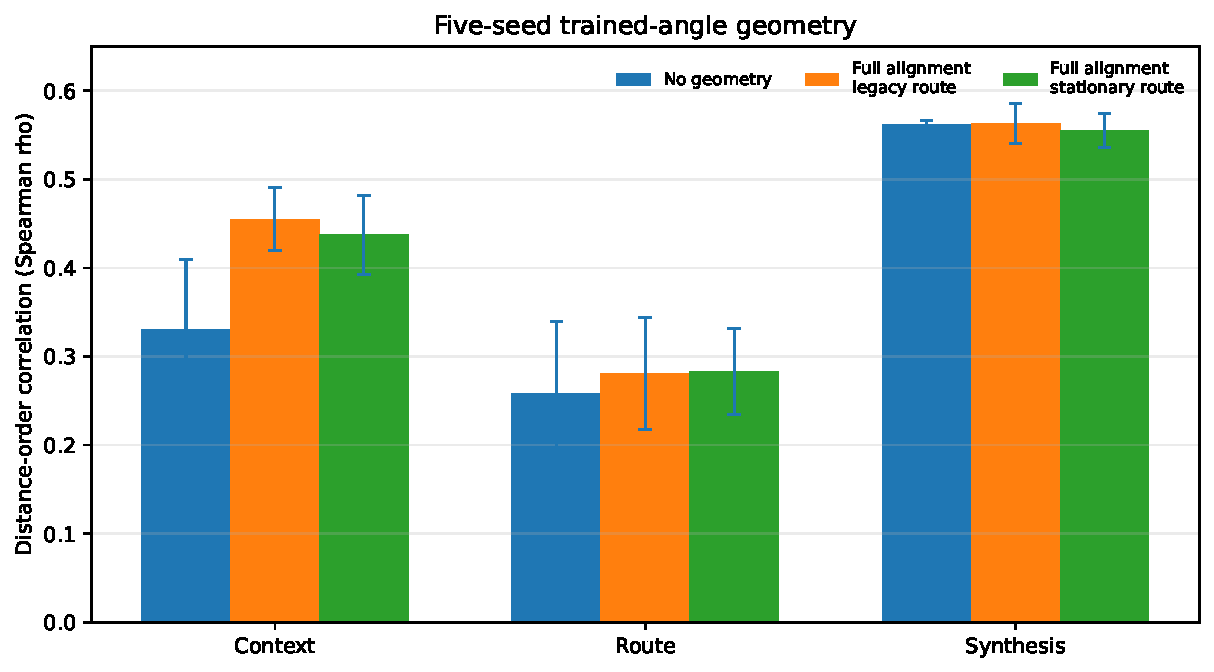
\includegraphics[width=0.92\textwidth]{../figures/geometry_summary_v109.pdf}
\caption{Five-seed trained-angle geometry. Error bars are 95\% intervals across model seeds. Context geometry improves under both full-alignment methods; route and synthesis effects are much weaker.}
\end{figure}

The stationary full-alignment model reaches mean context correlation $0.437$ versus $0.330$ for the no-geometry control. The paired seed effect is

\begin{equation}
 \Delta\rho_{\mathrm{context}}=+0.107,
 \qquad 95\%\ \mathrm{CI}=[+0.029,+0.185].
\end{equation}

Context stress decreases by $0.042$ with interval $[-0.084,-0.001]$. All five seeds have a positive context-order effect. This is the strongest result presently available.

\begin{figure}[H]
\centering
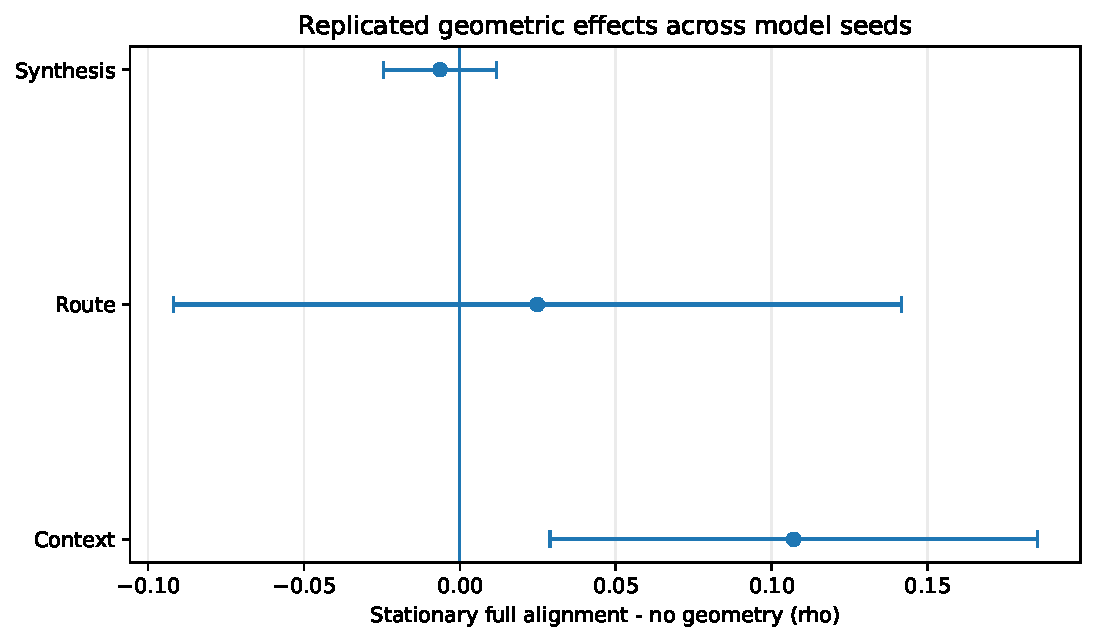
\includegraphics[width=0.78\textwidth]{../figures/seed_effects_v109.pdf}
\caption{Stationary full alignment minus no geometry. Only the context-order interval excludes zero.}
\end{figure}

\begin{positivebox}
\textbf{Reviewer-safe positive claim.} Across five matched-compute model seeds, the d4 aligned objective reproducibly increases trained-angle context distance-order correlation and reduces context stress on the controlled RotatedMNIST protocol.
\end{positivebox}

\subsection{Held-out source factor decoding improves}

\begin{figure}[H]
\centering
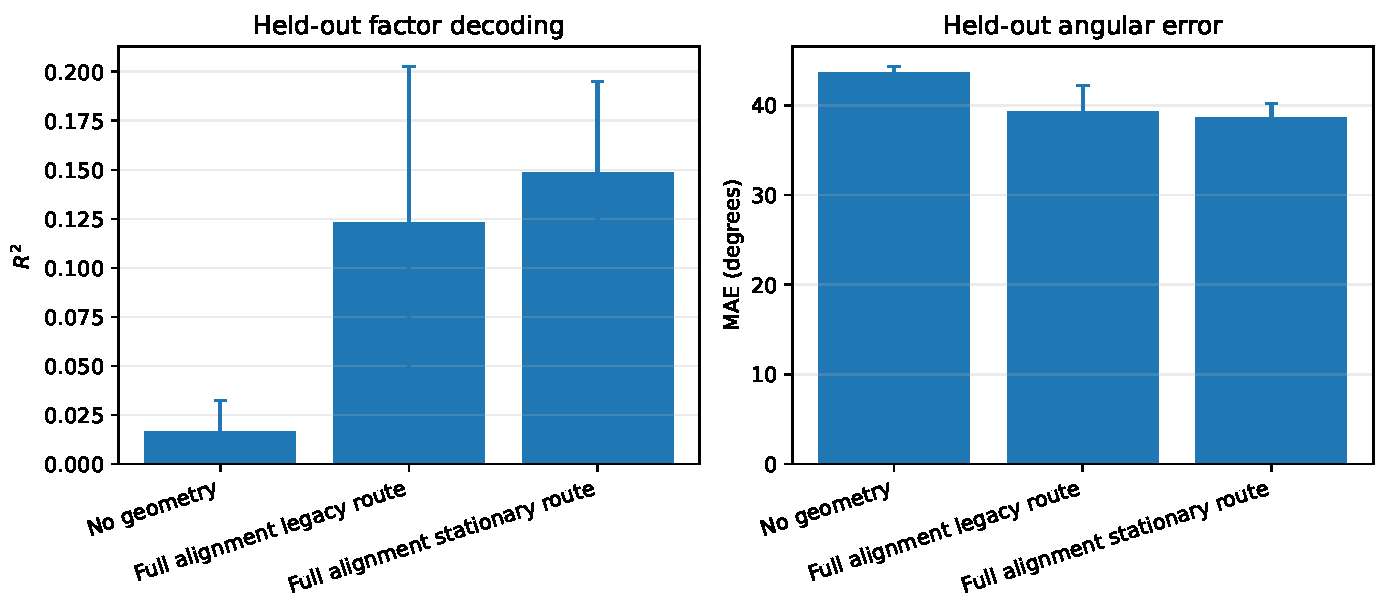
\includegraphics[width=0.94\textwidth]{../figures/heldout_decoding_v109.pdf}
\caption{Factor decoding on source identities excluded from tangent fitting. Full alignment improves context $R^2$ and reduces angular error, while the stationary and legacy route targets are statistically similar.}
\end{figure}

The stationary model improves held-out context $R^2$ from $0.016$ to $0.149$. The paired effect is $+0.132$ with seed interval $[+0.093,+0.172]$. Mean angular error falls from $43.67^{\circ}$ to $38.68^{\circ}$, a reduction of approximately $4.99^{\circ}$ with interval $[-6.35^{\circ},-3.63^{\circ}]$.

This result is important because evaluation uses unseen source identities. It argues against an interpretation in which the context merely memorizes source-specific trajectories.

\subsection{The stationary route target does not outperform the legacy target}

The direct stationary-minus-legacy effects are statistically neutral for context and route geometry:

\begin{center}
\begin{tabular}{lrrr}
\toprule
Metric & Mean effect & 95\% lower & 95\% upper \\
\midrule
Context $\rho$ & $-0.018$ & $-0.045$ & $+0.009$ \\
Route $\rho$ & $+0.003$ & $-0.034$ & $+0.039$ \\
Held-out context $R^2$ & $+0.026$ & $-0.037$ & $+0.088$ \\
Held-out accuracy & $-0.0005$ & $-0.0077$ & $+0.0067$ \\
Final trained accuracy & $-0.0006$ & $-0.0042$ & $+0.0030$ \\
Forgetting & $+0.0006$ & $-0.0028$ & $+0.0040$ \\
\bottomrule
\end{tabular}
\end{center}

The stationary target is still preferable as a specification because it is curriculum independent and numerically stable. However, empirical superiority is not supported. The replicated context result must be attributed to the broader d4 alignment package, not to the target replacement alone.

\subsection{Route geometry does not replicate}

The stationary route-order effect versus no geometry is $+0.025$ with interval $[-0.092,+0.142]$. Only two of five seeds are positive. On the dense held-out angle grid, the effect is $-0.006$ with interval $[-0.104,+0.093]$.

\begin{warningbox}
The five-seed evidence changes the interpretation of v1.0.8. Context geometry replicates; route geometry does not. The program currently has evidence for an ordered latent context representation, not a stable route manifold.
\end{warningbox}

\subsection{Synthesis geometry remains unchanged}

Stationary full alignment changes synthesis $\rho$ by $-0.006$ relative to no geometry, with interval $[-0.025,+0.012]$. Relative to the legacy route target, stationary routing reduces synthesis correlation by $0.0076$ with a fully negative interval and slightly worsens synthesis stress in every seed.

The desired chain

\begin{equation}
 \text{context geometry}\rightarrow\text{route geometry}
 \rightarrow\text{host synthesis geometry}
\end{equation}

is therefore not established. The current result remains representational rather than fully functional.

\subsection{Prediction and forgetting remain neutral}

\begin{figure}[H]
\centering
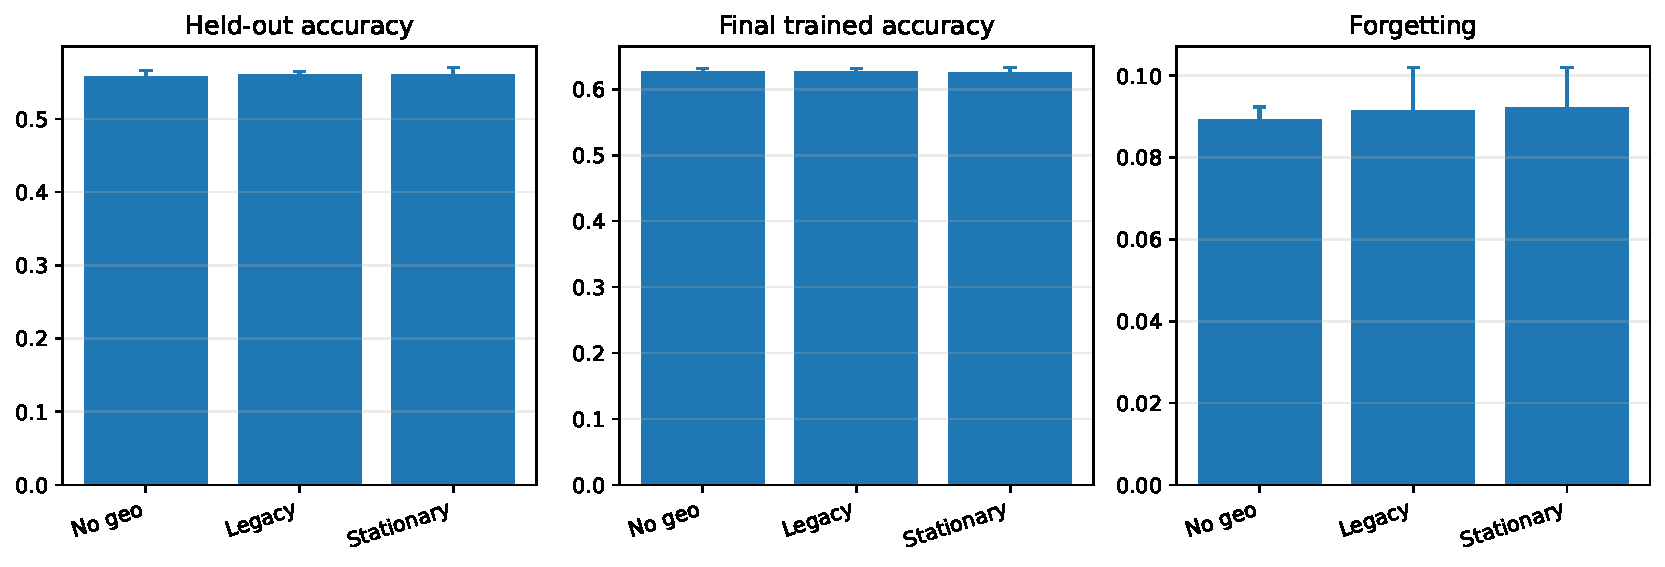
\includegraphics[width=0.98\textwidth]{../figures/operational_metrics_v109.pdf}
\caption{Operational metrics across five seeds. The small differences between methods are not statistically reliable.}
\end{figure}

\begin{table}[H]
\centering
\caption{Aggregate operational results.}
\begin{tabular}{lrrr}
\toprule
Method & Held-out accuracy & Final trained accuracy & Forgetting \\
\midrule
No geometry & 0.5583 & 0.6263 & \textbf{0.0894} \\
Legacy full alignment & \textbf{0.5612} & \textbf{0.6264} & 0.0916 \\
Stationary full alignment & 0.5607 & 0.6258 & 0.0922 \\
\bottomrule
\end{tabular}
\end{table}

Stationary full alignment changes held-out accuracy by only $+0.23$ percentage point, final trained accuracy by $-0.05$ point, and forgetting by $+0.28$ point. Every seed-level interval includes zero. C2 and C6 do not pass.

\subsection{Causal specificity does not replicate}

\begin{figure}[H]
\centering
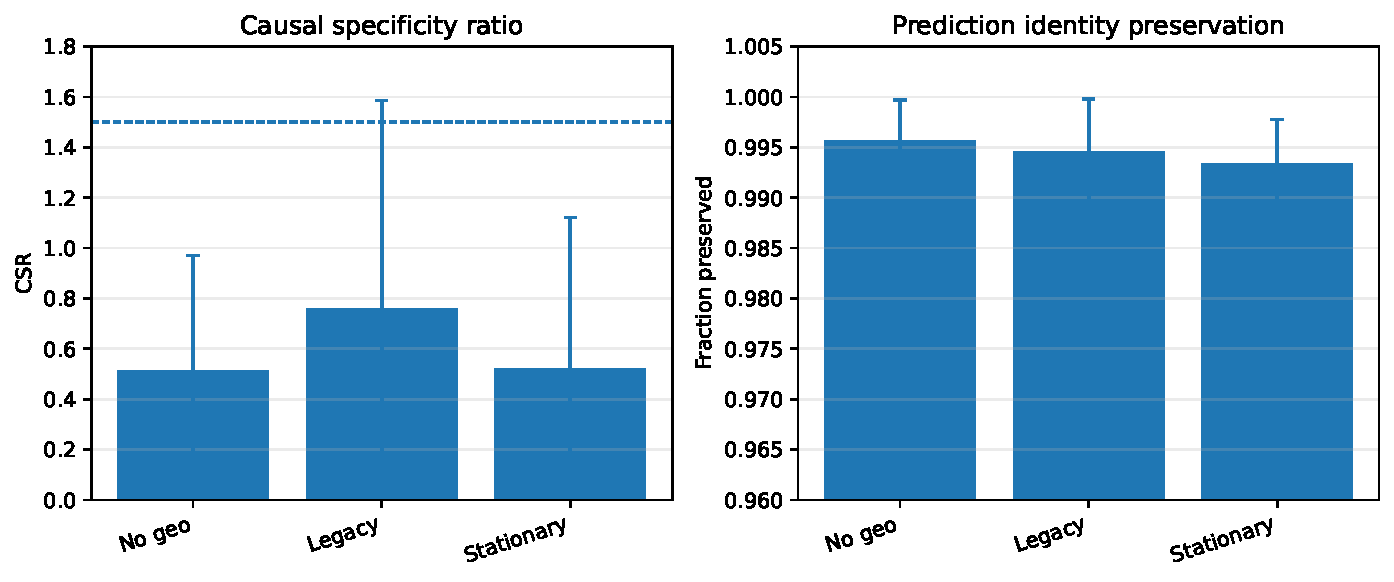
\includegraphics[width=0.94\textwidth]{../figures/causal_summary_v109.pdf}
\caption{Causal specificity and prediction preservation. Prediction identity is preserved, but CSR remains below the candidate threshold and varies strongly across seeds.}
\end{figure}

The stationary model has mean CSR $0.523$ with seed interval $[-0.075,1.121]$, well below the $1.5$ pilot threshold. Mean prediction identity preservation is high at $0.9934$, and true-class log-probability changes are small. Thus interventions are gentle but not factor-specific. The strong seed-0 v1.0.8 causal observation did not replicate.

\subsection{Per-seed heterogeneity}

\begin{figure}[H]
\centering
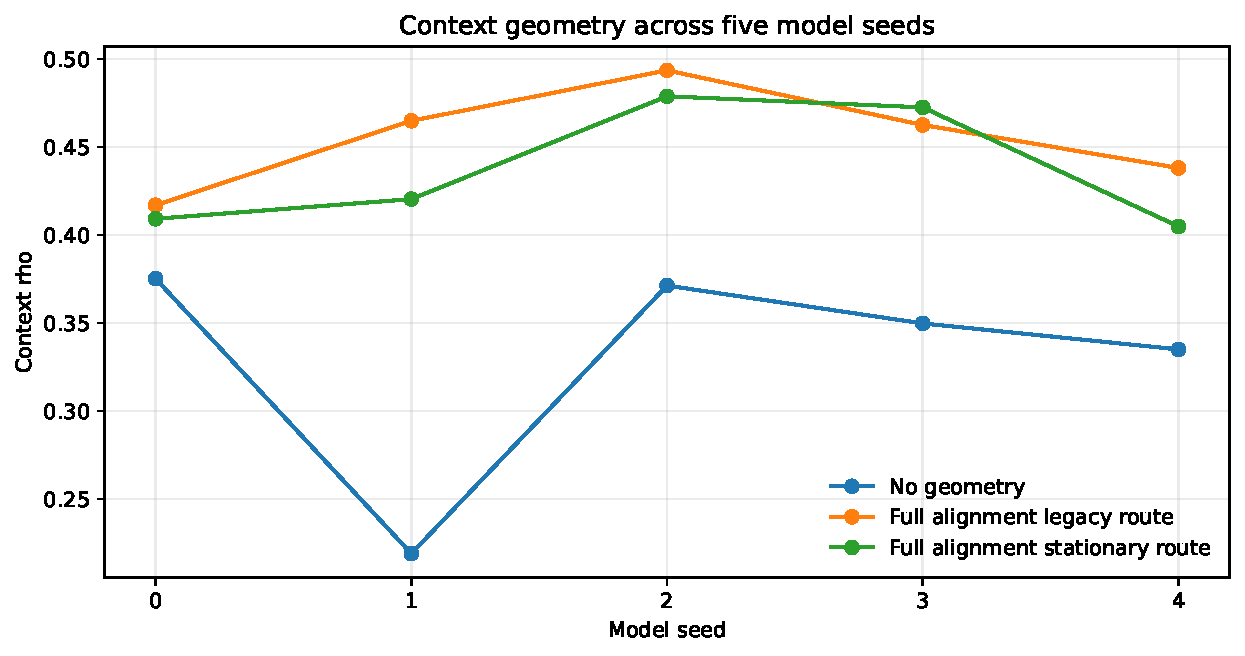
\includegraphics[width=0.88\textwidth]{../figures/per_seed_context_v109.pdf}
\caption{Context order by model seed. Full alignment improves context geometry in every seed, but effect magnitude varies substantially.}
\end{figure}

Five seeds are sufficient to identify a reproducible direction but not to estimate small effects precisely. Context-order improvement is robust in sign, while route, causal, and operational effects are dominated by between-seed variance.

\section{Integrated interpretation}

\subsection{What v1.0.9 establishes}

The pilot supports four narrow conclusions:

\begin{enumerate}
\item A context bottleneck can carry factor information when direct sensory shortcutting is prevented.
\item Four-dimensional local and cross-source alignment reproducibly improves context order and reduces context stress.
\item The learned context transfers factor information to unseen source identities.
\item The result is attributable to the complete context-alignment package rather than to the stationary route target alone.
\end{enumerate}

\subsection{What v1.0.9 falsifies or weakens}

The pilot weakens several tempting interpretations:

\begin{itemize}
\item Better context geometry does not automatically produce better route geometry.
\item Better context geometry does not automatically alter host synthesis.
\item A theoretically cleaner route target need not produce a stronger empirical result.
\item Single-seed causal specificity is not reliable evidence of C4.
\item Geometric correlation alone is not an operational objective.
\end{itemize}

\subsection{Representational geometry versus functional geometry}

The evidence now requires a sharper vocabulary.

\textbf{Representational geometry} means that internal context distances encode a controlled factor, remain noncollapsed, and generalize across source identities.

\textbf{Functional geometry} would additionally require that this structure causally governs routing, host transformations, synthesis, memory transport, or operational performance.

v1.0.9 supports the former at candidate level and does not yet support the latter.

\subsection{Why the result still matters}

A replicated positive latent-geometry result is scientifically useful even without accuracy gain. It establishes that the architecture and loss family can create stable factor structure rather than a projection artifact. It also narrows the next problem: the bottleneck is no longer basic representability, but functional coupling.

The failed operational bridge is equally informative. It prevents overclaiming and suggests that future work should optimize mediation and transport, not merely increase $\rho_{\mathrm{context}}$.

\section{What is established, promising, failed, or untested}

\begin{longtable}{p{0.27\textwidth}p{0.18\textwidth}p{0.47\textwidth}}
\toprule
Claim & Status & Evidence and qualification \\
\midrule
Executable matched-compute protocol & Established at development level & Five seeds completed; source and model seeds recorded; equal compute passed. \\
Context sufficiency under bottleneck & Strong development evidence & v1.0.7 interventions and competitive performance. \\
Replicated context geometry & Candidate pass & $\Delta\rho=0.107$ with positive seed CI; stress decreases; all five seeds positive. \\
Held-out context factor decoding & Promising replicated evidence & $\Delta R^2=0.132$ and about $5^{\circ}$ MAE reduction. \\
Stationary target superiority & Failed & Stationary-minus-legacy intervals include zero for primary geometry and operation metrics. \\
Replicated route geometry & Failed/inconclusive & Wide seed interval crossing zero. \\
Synthesis geometry & Failed/inconclusive & No improvement; stationary slightly worse than legacy. \\
Predictive utility & Failed/inconclusive & Accuracy intervals include zero. \\
Causal specificity & Failed & CSR below threshold and not replicated. \\
Host specialization & Untested in v1.0.9 & Requires dedicated ablation and cross-seed role matching. \\
Dual-memory transport & Untested & Current anchor is controlled rehearsal, not MMALS dual memory. \\
Operational utility & Not qualified & No reliable benefit in accuracy, forgetting, cost, or stability. \\
Domain-general geometry & Untested & Only controlled RotatedMNIST has been studied. \\
\bottomrule
\end{longtable}

\section{Reviewer risk assessment}

\subsection{Risk 1: supervised shaping may be mistaken for discovery}

The rotation angle is used in training losses. The paper must call the current protocol supervised geometric grounding. A later G1-B variant must exclude the factor from all losses before any claim of unsupervised context discovery.

\subsection{Risk 2: small number of model seeds}

Five seeds are enough to reveal a replicated positive direction but not enough to stabilize small route or operational effects. Any submission should report all seed values, Student-$t$ intervals, and positive-seed fractions rather than relying on a pooled sample-level $p$-value.

\subsection{Risk 3: controlled synthetic transformation}

Rotation provides unusually clean ground truth. The result may not transfer to overlapping classes, appearance drift, domain shift, or real temporal change. A second controlled factor and one non-synthetic domain are required before a general geometry claim.

\subsection{Risk 4: the factor may be decodable but functionally ignored}

The strongest current risk is that geometry is epiphenomenal. The classifier and host synthesis can solve the task without using the learned coordinate. Future protocols must explicitly test mediation and require function to depend on context.

\subsection{Risk 5: legacy and stationary route targets are not cleanly separable in effect}

Both full methods include the same context, fiber, and centroid terms. The target comparison is valid, but its effect is small relative to the broader alignment package. Claims must not attribute the replicated context result to the stationary target.

\subsection{Risk 6: memory claims remain premature}

The retention anchor uses old views already available in the paired batch. It is a controlled regularizer, not evidence for reconstructive or synthetic MMALS memory. C5 must remain unclaimed.

\subsection{Risk 7: host ecology remains absent from the replicated pilot}

A geometry paper about routes and hosts will face questions if host functions are not evaluated. Dedicated host contribution, replacement, locality, role matching, and seed stability remain necessary.

\section{Publication positioning}

\subsection{What can be published now}

Two publication forms are defensible.

\textbf{Protocol and status paper.} The full research history, evidence ladder, control logic, failure analysis, and v1.0.9 candidate result can support an arXiv technical report. Its central contribution would be methodological discipline for qualifying internal geometry in modular continual-learning systems.

\textbf{Narrow empirical note.} A shorter note could report the replicated context-order and held-out decoding result, explicitly framing it as supervised representational grounding on one controlled benchmark.

\subsection{What is required for a stronger empirical G1 paper}

A broader empirical paper should require:

\begin{enumerate}
\item a second factor or dataset;
\item an unsupervised or weakly supervised G1-B comparison;
\item explicit functional mediation from context to route and host behavior;
\item host specialization evidence across seeds;
\item continual transport and memory tests;
\item operational benefit or a clearly justified negative result;
\item frozen preregistered gates before qualification runs.
\end{enumerate}

\subsection{What should remain separate}

Energy-guided routing belongs to G2 and phase-aware or density-state routing to G3. These extensions should not be merged into the current empirical claim. The order remains

\begin{equation}
 \text{grounded geometry}\rightarrow
 \text{functional coupling}\rightarrow
 \text{energy-guided control}\rightarrow
 \text{phase-aware extensions}.
\end{equation}

\section{Recommended next experiments}

\subsection{Priority A: force functional use of context geometry}

The next model should not merely make factor information available. It should require the route or host system to use it. Candidate mechanisms include:

\begin{itemize}
\item remove or severely regularize direct sensory-to-router access;
\item predict route coordinates from context through a low-capacity map;
\item add a mediation loss measuring route dependence on context;
\item penalize successful prediction under context shuffling;
\item require host-selection changes to follow the context tangent.
\end{itemize}

\subsection{Priority B: couple geometry to host function}

A route can be geometrically ordered while hosts compensate for it arbitrarily. Introduce transition consistency:

\begin{equation}
 g_{r(u+\Delta u)}(z_0(u+\Delta u))
 \approx \mathcal{T}_{\Delta u}
 g_{r(u)}(z_0(u)),
\end{equation}

where $\mathcal{T}_{\Delta u}$ is a learned or known transport operator. This directly tests whether moving in context corresponds to a coherent functional transformation.

\subsection{Priority C: intervention-trained geometry}

Current causal probes are post hoc. A stronger design would train with local counterfactual consistency: perturb context along the learned factor tangent and require predictable route or synthesis movement while preserving class identity.

\subsection{Priority D: memory transport}

Replace direct old-view anchoring with bounded reconstructive and synthetic memory. Measure whether geometry, function, and predictions for old contexts can be reconstructed after later stages. This is the first legitimate C5 experiment.

\subsection{Priority E: domain breadth}

Replicate the same ladder on a second controlled factor such as scale, shear, illumination, or domain style, then on a real continual-learning dataset. The objective is not to maximize benchmarks immediately, but to test whether the geometry qualification method transfers.

\subsection{Priority F: qualification design}

Before the next multi-seed qualification run:

\begin{itemize}
\item freeze method variants and thresholds;
\item separate pilot-tuned from qualification data;
\item report all failed runs and numerical exceptions;
\item retain exact source, model, and intervention seeds;
\item map each manuscript claim to a CSV, figure, and gate.
\end{itemize}

\section{Anticipated reviewer questions and direct answers}

\subsection*{Did v1.0.9 prove that MMALS has a functional geometry?}

No. It produced replicated candidate evidence for context representation geometry. Route, synthesis, causal specificity, and operational utility did not replicate.

\subsection*{Is the result just supervised metric learning?}

The current G1-A protocol is supervised geometric grounding and should be described that way. The contribution is the controlled qualification of where the geometry appears and where it does not. Unsupervised discovery remains future work.

\subsection*{Why is the context result meaningful if accuracy is unchanged?}

Because the result establishes a stable internal relation that generalizes across source identities. It narrows the engineering problem from representability to mediation. It is not yet an operational success.

\subsection*{Did the stationary route target work?}

It worked numerically and removed curriculum-dependent target inconsistency. It did not outperform the legacy target empirically. The report treats this as a clean negative result.

\subsection*{Could the seed interval be optimistic with only five seeds?}

Yes. The interval is a pilot estimate and should not be presented as final qualification. The consistency of sign across five seeds is more informative than a precise small-sample interval.

\subsection*{Why not move directly to energy or quantum-inspired routing?}

Because the current geometry is not yet functionally coupled to routing and synthesis. Adding energy or phase structure now would multiply abstractions before the base causal chain is established.

\subsection*{What is the strongest reviewer-facing contribution now?}

A falsifiable evidence ladder plus a replicated narrow result: globally aligned d4 training produces a more ordered and more decodable context space, while several stronger interpretations fail under matched controls.

\section{Conclusion}

Geometry-MMALS G1 has moved beyond conceptual metaphor and single-run visualization. The v1.0.9 pilot provides the first replicated candidate evidence that the system can learn a grounded latent context geometry on a controlled continual-learning benchmark. The effect survives model seeds and transfers to held-out source identities. Equally important, the same pilot shows that route geometry, synthesis geometry, prediction, forgetting, and causal specificity do not improve reliably, and that a theoretically cleaner stationary route target is not empirically superior.

The reviewer-facing conclusion should therefore be calibrated but substantive: the program has demonstrated representational context geometry, not yet functional geometry. The next scientific task is to make route and host function depend causally on that geometry, then test whether the resulting structure survives continual transport, domain variation, and operational constraints.

\appendix

\section{Current gate table}

\begin{longtable}{p{0.42\textwidth}p{0.15\textwidth}p{0.33\textwidth}}
\toprule
Gate & Decision & Comment \\
\midrule
C0 equal compute across five seeds & Pass & 15,360 forwards and 80 optimizer steps per method and seed. \\
C1 stationary context $\rho$ seed interval & Candidate pass & Mean effect $+0.107$, interval $[+0.029,+0.185]$. \\
C1 stationary context stress & Candidate pass & Mean effect $-0.042$, interval $[-0.084,-0.001]$. \\
C1 route geometry & Fail/inconclusive & Interval crosses zero. \\
Stationary target beats legacy & Fail & Primary intervals cross zero. \\
Held-out factor decoding & Promising & $R^2$ and MAE improve across seeds. \\
C2 predictive superiority & Fail/inconclusive & Accuracy effects cross zero. \\
C3 host specialization & Not evaluated & Dedicated experiment required. \\
C4 source-bootstrap specificity & Fail & CSR below threshold. \\
C4 identity preservation & Candidate pass & Prediction preservation about 0.993. \\
C5 memory transport & Not implemented & Retention anchor is not dual memory. \\
C6 operational utility & Not qualified & No reliable accuracy, forgetting, or cost gain. \\
\bottomrule
\end{longtable}

\section{Reproducibility snapshot}

\begin{itemize}
\item Scientific version: Geometry-MMALS G1 v1.0.9.
\item Build revision: \texttt{stationary-route-qualification-pilot-r3}.
\item Model seeds: $0,1,2,3,4$.
\item Fixed source split and frozen sensory grove.
\item Sensory acceptance accuracy: approximately $0.942$.
\item Equal compute: 15,360 image forwards and 80 optimizer steps per method per seed.
\item Within-seed uncertainty: source-block bootstrap.
\item Across-seed uncertainty: Student-$t$ interval over model seeds.
\item Dense held-out angle grid: every $15^{\circ}$ from $-75^{\circ}$ to $+75^{\circ}$.
\item Execution-stability tests: non-negative RNG seed mapping; collapsed and near-collapsed route backward tests.
\item Archived evidence: aggregate tables, per-seed effects, causal summaries, run manifest, source hashes, and raw seed folders.
\end{itemize}

\section{Exact key evidence snapshot}

\begin{table}[H]
\centering
\caption{Stationary full alignment versus no geometry.}
\begin{tabular}{lrrr}
\toprule
Evidence & Mean effect & 95\% lower & 95\% upper \\
\midrule
Trained context $\rho$ & $+0.1071$ & $+0.0289$ & $+0.1852$ \\
Trained context stress & $-0.0423$ & $-0.0837$ & $-0.0010$ \\
Trained route $\rho$ & $+0.0248$ & $-0.0919$ & $+0.1415$ \\
Trained synthesis $\rho$ & $-0.0064$ & $-0.0246$ & $+0.0119$ \\
Dense held-out context $\rho$ & $+0.0484$ & $-0.0119$ & $+0.1088$ \\
Held-out context $R^2$ & $+0.1323$ & $+0.0930$ & $+0.1716$ \\
Held-out angular MAE & $-4.9889^{\circ}$ & $-6.3489^{\circ}$ & $-3.6289^{\circ}$ \\
Held-out accuracy & $+0.0023$ & interval crosses zero & -- \\
Final trained accuracy & $-0.0005$ & interval crosses zero & -- \\
Forgetting & $+0.0028$ & interval crosses zero & -- \\
\bottomrule
\end{tabular}
\end{table}

\printbibliography

\end{document}
